\documentclass[12pt,a4paper]{article}

\usepackage[T1]{fontenc}
\usepackage[brazilian]{babel}
\usepackage{lmodern}
\usepackage[margin=2.5cm]{geometry}
\usepackage{amsmath}
\usepackage{amssymb}
\usepackage{graphicx}
\usepackage{booktabs}
\usepackage{microtype}
\usepackage[hidelinks]{hyperref}
\usepackage{natbib}

\title{Relatório de Análise do Ozônio}
\author{Ananda Cristina Diniz}
\date{\today}

\begin{document}

\maketitle

\section{Introdução e Origem dos Dados}
Os dados analisados neste relatório são provenientes do conjunto de dados \texttt{airquality}, disponibilizados no material da disciplina em arquivo compacto, além de poder ser obtido no ambiente R \citep{Rcore}. O conjunto contém um total de 153 observações diárias relativas a medições de qualidade do ar.
A variável selecionada nesse estudo foi a \texttt{Ozone}, que possui um total de 37 valores ausentes (NAs).

\section{Resultados e Análise}
Como observado na Tabela~\ref{tab:resumo}, é apresentada a contagem de dias com medições válidas em cada mês analisado, além da média mensal.

\begin{table}[htbp]
    \centering
    \begin{tabular}{ccc}
        \toprule
        Mês & Média de Ozônio & Dias Medidos \\
        \midrule
        5 & 23, 61 & 26 \\
        6 & 29, 44 & 9 \\
        7 & 59, 12 & 26 \\
        8 & 59, 96 & 26 \\
        9 & 31, 45 & 29 \\
        \bottomrule
    \end{tabular}
    \caption{Média mensal e contagem de observações da variável Ozônio}
    \label{tab:resumo}
\end{table}

A média amostral apresentada na Tabela~\ref{tab:resumo} foi calculada pela Equação~\eqref{eq:media_amostral}:

\begin{equation}
\label{eq:media_amostral}
\bar{X} = \frac{\sum_{i=1}^{n} X_i}{n}
\end{equation}

Quando há a presença de valores ausentes (NAs) no conjunto de dados, o denominador $n$ contabiliza apenas a quantidade de dias que realmente foram medidos na amostra, desconsiderando as observações faltantes no cálculo.

A visualização da distribuição da variável Ozone foi gerada por meio do pacote de gráfico (\textit{ggplot}) do R \citep{ggplot2} e é apresentada na Figura~\ref{fig:distribuicao}.

\begin{figure}[htbp]
    \centering
    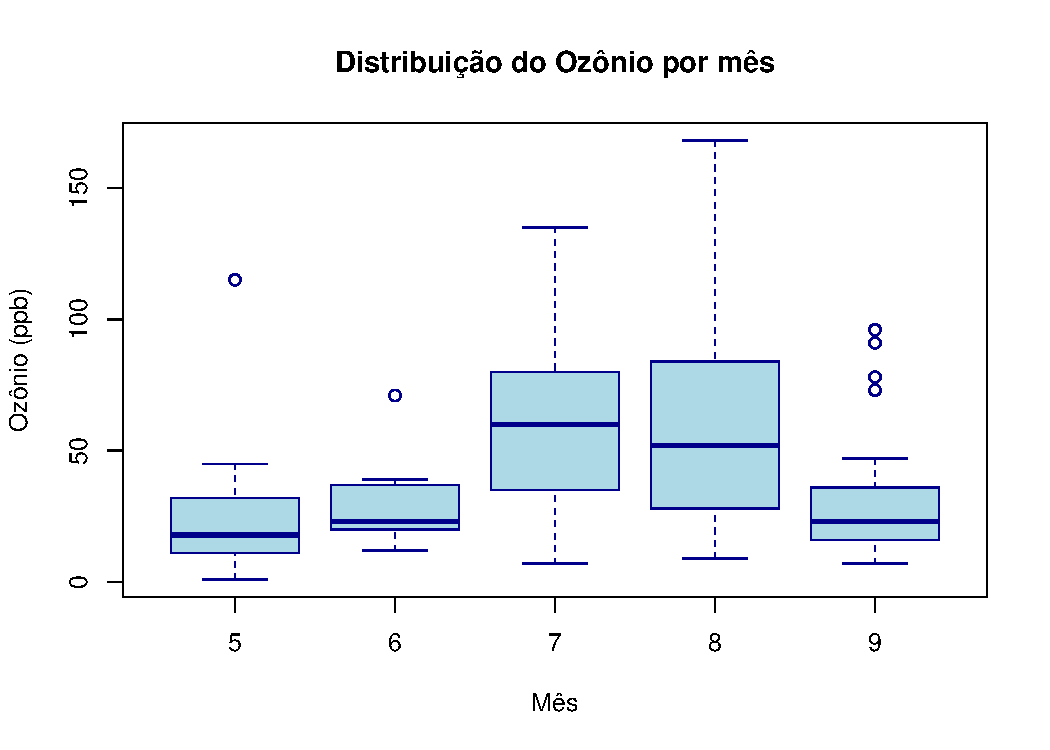
\includegraphics[width=0.75\linewidth]{figura.pdf}
    \caption{Distribuição dos níveis de Ozônio ao longo dos meses}
    \label{fig:distribuicao}
\end{figure}

\section*{Declaração de uso de IA}
A Inteligência Artificial Gemini foi utilizada para auxiliar na estruturação dos comandos LaTeX, correção de alguns comandos que estavam dando erro no terminal (e impossibilitava a realização da atividade) e verificação da sintaxe das citações. Todos os códigos gerados e resultados obtidos foram conferidos manualmente no terminal local.

\bibliographystyle{plainnat}
\bibliography{referencias}

\end{document}
